\section{証明}
\label{section:differentiable}

証明の概略を示す.
まず$\classPSPACE$または$\classCH$困難なある種の離散版の常微分方程式
を得る(\ref{section:divp}節, \ref{subsection: counting hierarchy}節).
そして離散版常微分方程式を模倣する, 滑らかな実関数族とその常微分方程式の解のペア $(g_u)_u, (h_u)_u$ の存在を示す(\ref{subsection: ode family}節).
それらを一つの滑らかな実関数へ埋め込むことで定理で求める $g, h$ を構成する(\ref{subsection: proof of theorems}節).

Lipschitz条件の場合の証明では用いられていない新たな技巧は2点ある.
1つは滑らかな多項式時間計算可能関数を用いて実関数を構成することにより
微分可能としたこと,
もうひとつは河村によって定義されたLipschitz連続な微分方程式の離散版を,
より形式的に定義し, さらに任意回微分可能な微分方程式の離散版を構成して
その$\classCH$困難性を示した点である.



\subsection{差分方程式}
\label{section:divp}

Lipschitz連続な常微分方程式の$\classPSPACE$困難性の証明では
最初のステップとして, まずの離散版の常微分方程式を定義し, 
それが$\classPSPACE$困難であることを示している
\cite[補題4.7]{kawamura2010lipschitz}.
この節では離散版微分方程式をより形式的に定義し,
滑らかな常微分方程式の離散版が$\classPSPACE$困難ないし$\classCH$困難であることを示す.

$[n] = \{0, \dots , n-1\}$ と表記する.
関数 $G \colon [P] \times [Q] \times [R] \to \{-1, 0, 1\}$ に対して,
関数 $H \colon [P + 1] \times [Q+1] \to [R]$ が
任意の $i \in [P],\ T \in [Q]$ について以下を満たすとき,
$H$ を $G$ の\emph{差分方程式}の解と呼ぶ.
\begin{gather}
   H(i, 0) = H(0, T) = 0 \label{eq:initial value}
\\
   H(i + 1, T + 1) - H(i+1, T) = G(i, T, H(i, T))  \label{eq:divp}
\end{gather}
$P, Q, R$ をそれぞれ\emph{段数}, \emph{列数}, \emph{欄の大きさ}と呼ぶ.
常微分方程式(\ref{eq:ode})の1つめの条件($h(0) = 0$)と式(\ref{eq:initial value}),
2つめの条件($\D h(t) = g(t, h(t))$)と式(\ref{eq:divp})
の間に対応関係を見て取ることができるため,
差分方程式は常微分方程式の離散版と呼べる(図 \ref{fig:divp}).

文字列 $u$ ごとに一つの差分方程式 $G _u$ を与え,
$u$が言語$L$に入っているかをその差分方程式によって計算することを考える.
各 $u$ に対して $G_u$ の段数と列数, 解をそれぞれ $P_u, Q_u, H_u$ としたとき,
言語 $L$ が関数族 $(G_u)_u$ によって認識されるとは,
$H_u(P_u, Q_u) = L(u)$ を満たすこととする.
ここで言語 $L \subseteq \{0, 1\} ^*$ は
関数 $L \colon \{0, 1\} ^* \to \{0, 1\}$ と同一視し, 
$u \in L$ のとき $L (u) = 1$ としている. 

 \begin{figure}
  \label{fig:divp}
  \begin{center}
   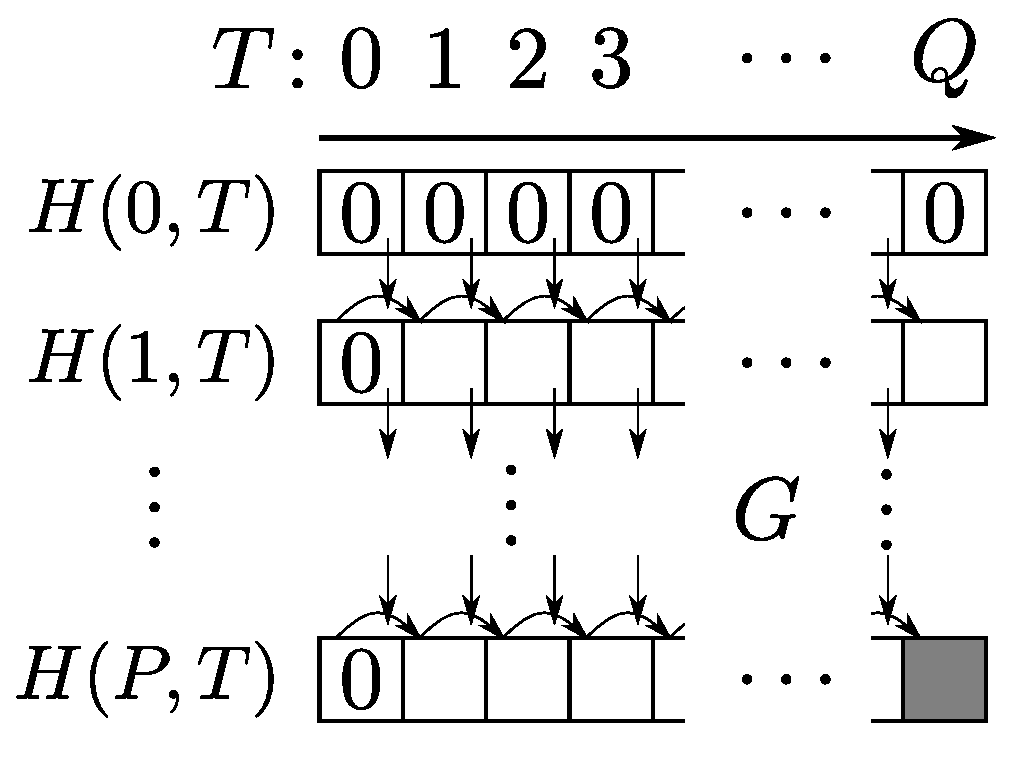
\includegraphics[height=0.2\textheight]{image/divp.eps}
  \end{center}
  \caption{差分方程式と認識される言語}
 \end{figure}

このままでは任意の言語を差分方程式で認識可能となってしまうので, $(G_u)_u$全体にある種の制限をかける.
$(G_u)_u$ が{\bf 一様}であるとは,
各 $u$ について $G _u$ の段数, 列数及び欄の大きさが $|u|$ の多項式の指数($2^{\mathrm{poly} (|u|)}$)で抑えられ, 
かつ与えられた $(u, i, T, Y)$ から多項式時間で $G_u(i, T, Y)$ が
計算できることと定義する.

$G_u$ の段数がさらに $|u|$ の多項式, 対数で抑えられるとき, 
族 $(G_u) _u$ はそれぞれ\emph{多項式段}, \emph{対数段}であるという. 
河村の論文では次が示されている.
\begin{lemma}[{\cite[補題4.7]{kawamura2010lipschitz}}]
 \label{DIVPpolyIsPSPACEhard}
 $\classPSPACE$ 困難で多項式段一様な関数族によって認識される言語が存在する
 \footnote{差分方程式によって認識される言語のクラスはカープ還元において閉じており,
多項式段一様な関数族によって認識される言語は$\classPSPACE$と一致する.}.
\end{lemma}
$g$ が $(\infty, 1)$ 回微分可能であるときも,
この補題を用いて$\classPSPACE$困難な常微分方程式の解を構成することができる.
2回以上微分可能な関数によって与えられるの常微分方程式の計算量を考えるとき,
その滑らかさの制限により多項式段の差分方程式を模倣することができなかった.
しかし差分方程式を対数段に制限してやれば模倣可能である
(\ref{subsection: ode family}節, \ref{subsection: proof of theorems}節).
そこで対数段一様な差分方程式の困難性について注目し以下の結果を得た.
\begin{lemma}
 \label{DIVPlogIsCHhard}
 $\classCH$ 困難で対数段一様な関数族によって認識される言語が存在する.
\end{lemma}
計数階層$\classCH$の定義及びこの補題の証明は次章にて行う.

\subsection{計数階層と対数段差分方程式}
\label{subsection: counting hierarchy}

\emph{計数階層}(Counting Hierarchy($\classCH$)) とは
Wagner によって導入された計算量クラスである\cite{wagner1986complexity}.
多項式階層({\bf PH})が {\bf NP} の神託機械を用いて,
\begin{align*}
 \Sigma^p_0  &= \classP
 \\
 \Sigma^p_{k+1} &= \mathbf{NP}^{\Sigma^p_k}
 \\
 \mathbf{PH} &= \bigcup_k \Sigma^p_k
\end{align*}
と定義されるのに対し,
計数階層は多項式階層の {\bf NP} を {\bf PP} で置き換えたものである
\footnote{ただしこの特徴付けは Tor{\'a}n によるものであり,
Wagner によるオリジナルの定義とは異なる\cite{toran1991complexity}.
}. つまり
\begin{align*}
 \C_0 \classP  &= \classP
 \\
 \C_{k+1} \classP &= \classPP^{\C_k \classP}
 \\
 \classCH &= \bigcup_k \C_k \classP.
\end{align*}

$\mathbf{PH} \subseteq \classCH \subseteq \classPSPACE$ だが,
いずれの包含関係も厳密か否かは未解決である.

補題 \ref{DIVPlogIsCHhard} における $\classCH$困難な言語を定義するため, 
まず$\classCH$ の各階層 $\C_n \classP$ に対する完全問題$\C_n B_{be}$を導入する.
論理式を真にする割り当ての数が一定以上であれば真となる量化子を考える.
つまり量化子 $\C$ を自然数 $m$, $l$ 個の論理変数の組 $X$,
論理式 $\phi(X)$について以下のように定義する.
\begin{equation}
 \C^m X \phi(X) 
  \longleftrightarrow 
  \Bigl|\{X \in \{0, 1\}^l \mid \phi(X) = 1\}\Bigr| \ge m.
\end{equation}
$\C^1 = \exists$, $\C^{2^l} = \forall$ であり, $\C$ は $\exists, \forall$ の
一般化と言える.
言語 $\C_n B_{be}$ を以下のように定義する.
\begin{equation}
 \langle \phi(X_1, \dots, X_n), m_1, \dots, m_n \rangle \in \C_n B_{be}
 \longleftrightarrow
 \C^{m_1}{X_1} \cdots \C^{m_n}{X_n} \phi(X_1, \dots, X_n) 
\end{equation}
ただし $\langle \cdot \rangle$ は組み合わせ関数,
$X_i$ は $l_i$ 個の論理変数の組,
$\phi(X_1, \dots, X_n)$は$X_1, \dots, X_n$以外の変数を持たない論理式とする.


\begin{lemma}[{\cite[定理 7]{wagner1986complexity}}] \label{lemma:CnP-complete}
 $\C_n B_{be}$ は $\C_n\classP$ 完全.
\end{lemma}


$(\C_n B_{be})_n$ をまとめた言語 $\C_{\log} B_{be}$ を以下のように定義する.
\begin{equation}
 \langle 0^{2^n}, u \rangle \in \C_{\log} B_{be}
 \longleftrightarrow
 u \in \C_n B_{be}
\end{equation}
入力として階層の指数サイズ($0^{2^n}$)を与えているのは,padding することで
段数を入力長の対数オーダーとすることで, 対数段の差分方程式により認識可能とするためである.
この $\C_{\log} B_{be}$ が補題 \ref{DIVPlogIsCHhard} で求める言語であること,
つまり$\classCH$困難かつ対数段一様関数族によって認識可能であることを示す.


\begin{proof}[\rm 補題 \ref{DIVPlogIsCHhard} の証明]
 $\C_{\log} B_{be}$が$\classCH$困難であることを示す.
 任意の $\classCH$ の言語 $A$ はある階層 $\C_n \classP$ に属する. 
 補題 \ref{lemma:CnP-complete} より任意の $u \in \{0,1\}^*$ について
 $u \in A \leftrightarrow f(u) \in \C_n B_{be}$ 
 を満たす多項式時間関数 $f$ が存在する.
 \begin{align}
  u \in A 
  & \longleftrightarrow \langle 0^{2^n}, f(u) \rangle \in \C_{\log} B_{be}
 \end{align}
 $n$ は定数であるため $\langle 0^{2^n}, f(\cdot) \rangle$ は多項式時間関数.
 よって $A$ は $\C_{\log} B_{be}$ に多項式時間還元可能.


 $\C_{\log} B_{be}$を認識する関数族 $(G_u)_u$, 
 その解$(H_u)_u$, 関数 $p \colon \N \to \N$, 多項式 $q,r$ を構成する.
 自然数 $n, m_1, \dots, m_n$, 論理式$\phi$を
 $u  = \langle 0^{2^n}, 
 \langle \phi(X_1, \dots, X_n), m_1, \dots, m_n \rangle \rangle$
 を満たすものとする. 
 (そのような$n, m_1, \dots, m_n, \phi$が存在しないとき$u \not \in A$.)
 
 
 $L = \C_{\log} B_{be}$,
 $l_i = |X_i|$,
 $s_i = \sum^i_{j=1}l_j + 2i$  と表記する.
 関数 $C^m \colon \N \to \N$ を
 \begin{equation}
  C^m(x) 
     = \begin{cases}
       1 & (x \ge m) \\
       0 & (x < m) \end{cases}
 \end{equation}
 と定義する. 
 任意の $i = 0, \dots, n$ と $n-i$ 個の文字列 
 $Y_{i+1} \in \{0,1\}^{l_{i+1}}, \dots, Y_n \in \{0,1\}^{l_n}$ 
 について論理式
 $\C^{m_{i}}{X_i} \cdots \C^{m_1}{X_1}
 \phi(X_1, \dots, X_i, Y_{i+1}, \dots, Y_n)$
 の真偽値を $\phi_i(Y_{i+1}, \dots, Y_n)$ と表記する.
 \begin{align}
  \phi_0 (Y_1, \dots, Y_n) &= \phi(Y_1, \dots, Y_n)
  \\ \label{eq:phi-step}
  \phi_{i+1}(Y_{i+2}, \dots, Y_n) 
  &= C^{m_{i+1}}\left(\sum\nolimits_{X_{i+1} \in \{0,1\}^{l_i}} 
  \phi_i(X_{i+1}, Y_{i+2}, \dots, Y_{n})\right) 
  \\
  \phi_n() &= L(u) 
 \end{align}
 $T \in \N$ に対し, $T_i$ を $T$ の2進表記における $i$ 桁目, 
 $T_{[i,j]} = T_{j-1} T_{j-2} \cdots T_{i+1} T_{i}$ と表記する.


 $G_u$ を $(i, T, Y) \in [n+1] \times [2^{s_n}+1] \times [2^{|u|}]$ の範囲で
 を以下のように定義する. 一段目つまり $i=0$ ならば
 \begin{equation}
  G_u(0,T,Y) = 
   (-1)^{T_{s_1}}\phi(T_{[1,s_1]}, T_{[s_1+1,s_2]},
    \dots, T_{[s_{n-1}+1,s_n]}) 
 \end{equation}
 $i \ge 1$ ならば
 \begin{equation} \label{eq:def-Gu:case0}
  G_u(i,T,Y) = 
   \begin{cases}
    (-1)^{T_{s_{i+1}}} C^{m_i}(Y) 
    & (T_{[1,s_i]} = 10 \cdots 0) \\
    0 & (\text{othewise}).
   \end{cases} 
 \end{equation}


 任意の $i \in [n+1]$, $T \in [2^{s_n}+1]$ について,
 $H_u(i,T) \in [2^{l_i}+1]$ が成りたつこと,
 および $T_{[1,s_i]} = 10 \cdots 0$ ならば
 \begin{equation} \label{eq:subformula}
  G_u(i,T,H_u(i,T)) = (-1)^{T_{s_{i+1}}} 
   \phi_i(T_{[s_i+1, s_{i+1}]}, \dots, T_{[s_{n-1}+1, s_n]})
 \end{equation}
 を満たすことを $i$ についての帰納法により示す.
 上記が成り立つとき,
 $i=n$, $T=2^{s_n}$ において $G_u(n, 2^{s_n}, H_u(n,2^{s_n})) = \phi_n() = L(u)$
 よって $H_u(n+1, 2^{s_n}+1) = L(u)$.
 ここで 
 \begin{gather}
  n+1 \le \log(|0^{2^n}|) + 1 = O(\log(|u|)) \\
  2^{s_n}+1 \le 2^{s_n+1} \le 2^{|u|}
 \end{gather}
 より $p(u) = n+1, q(x) = r(x) = x$ とおき $G_u$ を
 $[p(u)] \times [2^{q(|u|)}] \times [2^{r(|u|)}]$ の範囲に拡張すると
 $H_u(p(u), 2^{q(|u|)}) = L(u)$.

 $i=0$ のとき, 式(\ref{eq:def-Gu:case0})より成り立つ.
 $i=j$ のとき, 成り立つと仮定する, $Y = H_u(i+1, T)$ とおくと
 \begin{align}
  Y 
  &= \sum_{V = 1}^{T-1} G_u(i, V, H_u(i, V)) \\
  &= \sum (-1)^{V_{s_{i+1}}} \phi_i(V_{[s_i+1, s_{i+1}]}, 
   \dots, V_{[s_{n-1}+1, s_n]})
 \end{align}
 $T_{[1, s_{i+1}]} = 10 \cdots 0$ のとき,
 $V_{[1, s_n]} = T_{[s_{i+1}+1,s_n]} 0 X 1 0 \cdots 0$ であるとき
 以外の値は打ち消し合うので,
 \begin{equation}
  Y = \sum\nolimits_{X \in \{0,1\}^{l_i}} 
  \phi_i(X, T_{[s_{i+1}+1, s_{i+2}]}, \dots, T_{[s_{n-1}+1, s_n]})
 \end{equation}
 式(\ref{eq:phi-step})より
 \begin{align}
  G_u(i+1,T,H_u(i+1,T)) 
  &= (-1)^{T_{s_{i+2}}} C^{m_{i+1}} (Y)\\
  &= (-1)^{T_{s_{i+2}}} \phi_{i+1}(T_{[s_{i+1}+1, s_{i+2}]}, \dots, T_{[s_{n-1}+1, s_n]})
 \end{align}
 よって $i=j+1$ でも成り立つ.
 \end{proof}



\subsection{差分方程式を模倣する関数族}
\label{subsection: ode family}
次に前節で示した$\classPSPACE$または$\classCH$困難な各差分方程式を滑らかな実関数で模倣可能であることを示す.

しかし補題を述べる前に実関数の多項式時間計算可能性を
実関数族のそれに拡張する.
文字列$u$で添字づけられた実関数$f _u \colon A \to \R$の
族 $(f_u)_u$ を機械 $M$ が計算するとは,
任意の実数 $x \in A$, 任意の $x$ の名 $\phi_x$ に対して,
文字列 $v$ を $M ^{\phi _x} (u, v)$ へ移す関数が, 
$f _u (x)$ の名であることをいう.
実関数族が多項式時間計算可能であるとは, その実関数族を計算する
多項式時間神託機械が存在することである.

 \begin{lemma}
  \label{KTimesFamily}
  或る $\classCH$ 困難な言語 $L$,
  二変数多項式 $\mu$ において,
  任意の正の整数 $k$,
  任意の多項式 $\gamma$ に対して,
  多項式 $\rho$, 実関数族 $(g_u)_u, (h_u)_u$ で, 
  $(g_u)_u$ は多項式時間計算可能であり,
  各文字列 $u$ に対して以下を満たすものが存在する.

  \begin{enumerate}
   \item \label{enum:kf:start}
     $g_u\colon [0,1] \times [-1,1]\to \R, \quad h_u\colon [0,1] \to [-1,1]$; 
   \item $h_u$ は $g_u$ の常微分方程式 (\ref{eq:ode}) の解;
   \item $g_u$ は $(\infty, k)$ 階連続微分可能;
   \item \label{enum:boundary}
	 任意の $i \in \N$, $y \in [-1,1]$ に対して
	 \begin{equation*}
	  \D^{(i, 0)} g_u(0,y) = \D^{(i, 0)} g_u(1,y) = 0 ;
	 \end{equation*}
   \item \label{enum:inftyk}
	 任意の $i \in \N$, $j \in \{0, \dots, k\}$ に対して
	 \begin{equation*}
	  \left|\D^{(i,j)} g_u(t,y)\right| \le 2^{\mu(i, |u|) - \gamma(|u|)};
	 \end{equation*}
   \item \label{enum:kf:end}
	 $h_u(1) = 2^{-\rho(|u|)}L(u)$.
  \end{enumerate}
 \end{lemma}

\begin{lemma}
 \label{DifferentiableFamily}
 或る $\classPSPACE$ 困難な言語 $L$,
 二変数多項式 $\mu$ において,
 $k = 1$のとき,
 任意の多項式 $\gamma$ に対して,
 多項式 $\rho$, 実関数族 $(g_u)_u, (h_u)_u$ で, 
 $(g_u)_u$ は多項式時間計算可能であり,
 各文字列 $u$ に対して
 補題\ref{KTimesFamily}の(\ref{enum:kf:start}) -- (\ref{enum:kf:end})を満たすものが存在する.
\end{lemma}



 この補題より各 $h_u$ が $g_u$ の常微分方程式の解であり, 
 各$h_u(1)$ に $L(u)$ の情報を持つ
 滑らかな実関数族 $(g_u)_u, (h_u)_u$ の存在が示される.
 河村によるLipschitz連続な常微分方程式の$\classPSPACE$困難性の証明における,
 補題4.1 に対応するが,
 $g$ を微分可能にするため, 条件 (iii) -- (v) が付け加えられている.


 この補題の証明の基本的な流れを説明する.
 任意の言語 $L \in \classPSPACE$ (resp. ある$\classCH$困難な言語$L$)に対し, 
 補題 \ref{DIVPpolyIsPSPACEhard}(resp. 補題 \ref{DIVPlogIsCHhard})
 を用いて $L$ を認識する $(G_u)_u$ 
 及びその差分方程式の解 $(H_u)_u$ を得る.
 そして各 $G_u, H_u$ を模倣する
 滑らかな $g_u \colon [0,1] \times [-1, 1] \to \R$ 
 とその常微分方程式の解 $h_u \colon [0,1] \to \R$ を構成する.
 また $(G_u)_u$ の一様性から $(g_u)_u$ の多項式時間計算可能性を示す.

 上記の証明は基本的に, 河村による証明と変わらない\cite[補題4.1]{kawamura2010lipschitz}.
 河村の証明と異なる点は, $g_u$ を滑らかな関数にするため, 
 以下のような無限回微分可能な多項式時間実関数 $f \colon [0,1] \to \R$ を用いて
 $g_u$ を構成していることである.

 \begin{lemma}[{\cite[補題 3.6]{ko1991complexity}}]
  \label{SmoothFunction}
  以下を満たす多項式時間計算可能で無限回微分可能な
  実関数 $f \colon [0,1] \to \R$ が存在する.

  \begin{enumerate}
   \item $f(0) = 0, \quad f(1) = 1$;
   \item 任意の $n \ge 1$ で $f^{(n)}(0) = f^{(n)}(1) = 0$;
   \item $f$ は $[0,1]$ で単調増加;
   \item 任意の $n \ge 1$ で $\D^n f$ は多項式時間実関数.
  \end{enumerate}
 \end{lemma}

 さらにここでは上記の条件に加えて, 
 \begin{enumerate}
  \setcounter{enumi}{4} 
  \item 以下を多項式 $s$が存在
	\begin{equation} \label{enum:polynomial-size}
	 |\D^n f| \le s(n)
	\end{equation}
 \end{enumerate}
 を満たすような$f$が存在することを用いて証明する.
 そのような$f$が存在することは葛による証明を確認することで容易に示される.

 ここではより難しく一般的な補題 \ref{KTimesFamily} のみ証明を行い,
 補題 \ref{DifferentiableFamily} については$g, h$の例のみ示し
 証明は省略する.
 \begin{proof}[\rm 補題 \ref{KTimesFamily} の証明]
  補題 \ref{DIVPlogIsCHhard} より
  $\classCH$ 困難な言語 $L$ を認識する
  対数段一様関数族 $(G_u)_u$, その解 $(H_u)_u$, 
  $P_u = p(|u|), Q_u = 2^{q(|u|)}, R_u = 2^{r(|u|)}$ を満たす関数$p$, 
  多項式 $q,r$ を得る.
  河村による証明と同様に
  以下のことを仮定する.
  \begin{gather}
   H_u(i, 2^{q(|u|)}) = \begin{cases}
			L(u) & (i=p(|u|)) \\
			0 & (i<p(|u|)).
			\end{cases}
   \\
   i \not = j_u(T)  \to G_u(i, T, Y) = 0 
  \end{gather}
  

 $B = 2^{\gamma(|u|) + r(|u|) + s(k) + k + 3}$ とおき, 
 各 $(t, y) \in [0,1] \times [-1, 1]$ に対して,
 自然数 $N$, $\theta \in [0,1]$, 整数 $Y$, $\eta \in [-1/4, 3/4]$ を
 $t = (T + \theta)2^{-q(|u|)}$, $y = (Y + \eta)B^{-(k+1)^{j_u(T)}}$ を満たすように
 定める.
  そのとき,
 \begin{equation}
  \delta_{u, Y} (t) = \frac{2^{q(|u|)} \D f(\theta)}{B^{(k+1)^{j_u(T)+1}}} 
   G_u\left( j_u(T),\ T,\ Y \bmod 2^{r(|u|)} \right)
 \end{equation}
 とおき $g_u, h_u$ を以下のように定義する.
 \begin{equation}
  \label{eq:gu}
\\  g_u(t,y) 
  = \begin{cases}
     \delta_{u, Y}(t)
     & (\eta \le \frac 1 4)
     \\
     ( 1-f ( \frac{4\eta-1}{2})) \delta_{u, Y}(t) 
     + f ( \frac{4\eta-1}{2}) \delta_{u,Y+1}(t)
     & (\eta > \frac 1 4)
    \end{cases}
 \end{equation}
 \begin{equation} 
  h_u(t) 
   = \sum^{p(|u|)}_{i=0} \frac{H_u(i, T)}{B^{(k+1)^i}}  
  + \frac{f(\theta)}{B^{(k+1)^{j_u(T)+1}}} G_u(j_u(T), T, H_u(j_u(T), T)) 
  \label{eq:hu}
 \end{equation}
  ただし$f$と多項式$s$は補題 \ref{SmoothFunction}
  および式(\ref{enum:polynomial-size})を満たすものとする.
  また$\rho(x) = 2^{p(x)} \cdot (\gamma(x) + r(x) + 3)$, 
  $\mu(x, y) = (x+1)q(y) + s(x+1)$とおく.


 上記のように定義した $g_u, h_u$ が補題\ref{DifferentiableFamily} で求める
 性質を満たすことを示す. ただし多くは河村による証明と同様に示せるため
  異なる条件 (iii) - (v) のみ示す
 
  $g_u$ が $(\infty, k)$ 階連続的微分可能であることを示す.
  $\eta$ が $[-1/4, 1/4]$ と $[1/4, 3/4]$ である区間それぞれにおいて微分する.
  任意の $i \in \N$ について

  \begin{equation}
   \D^i \delta_{u,Y}(t) 
    = \frac{2^{(i+1)q(|u|)} \D^{i+1}f(\theta)}{B^{(k+1)^{j_u(T)+1}}}
    G_u\left( j_u(T),\ T,\ Y \bmod 2^{r(|u|)} \right)
  \end{equation}

  \begin{equation}
   \label{eq:derivativeofgu}
    \D^{(i,0)} g_u(t, y)
     = \begin{cases}
 	\D^i \delta_{u, Y}(\theta) 
	\hfill (- \frac 1 4 < \eta < \frac 1 4) \\
	\left( 1-f \left(\frac{4\eta-1}{2}\right)\right) 
	\D^i \delta_{u, Y}(\theta) 
	+ f \left(\frac{4\eta-1}{2}\right) \D^i \delta_{u,Y+1}(\theta) \\
	\hfill (\frac 1 4 < \eta < \frac 3 4)
       \end{cases}
  \end{equation}   
  $j \in \{1, \dots , k\}$ について,

  \begin{equation}
    \D^{(i,j)} g_u(t, y)
     = \begin{cases}
	0 \hfill (- \frac 1 4 < \eta < \frac 1 4) \\
	(2B^{(k+1)^{j_u(T)}})^j \D^j f(\frac{4\eta - 1}2)
	(\D^i \delta_{u,Y+1}(\theta)-\D^i \delta_{u, Y}(\theta)) \\
	\hfill (\frac 1 4 < \eta < \frac 3 4)
       \end{cases}
  \end{equation}
  境界においても連続であるため,
  $g_u$ は $(\infty, j)$ 階連続的微分可能であることが示された.
  式 (\ref{eq:derivativeofgu}) に $t = 0, 1$ ($\theta = 0$) を代入して
  $\D^{(i, 0)} g_u(0,y) = \D^{(i, 0)} g_u(1,y) = 0$.
  上記の式より任意の $i \in \N$, $j \in \{0, \dots, k\}$ について
  $|\D^{(i,j)} g_u| \leq 2^{\mu(i, |u|) - \gamma(|u|)}$.

 \end{proof}

 補題 \ref{DifferentiableFamily} の証明では
 $\classPSPACE$困難な言語を認識する多項式段一様関数族$(G_u)_u$とその解$(H_u)_u$に対して
 \begin{align}
  \delta_{u, Y} (t) &= \frac{2^{q(|u|)} \D f(\theta)}{B^{{j_u(T)+1}}} 
   G_u\left( j_u(T),\ T,\ Y \bmod 2^{r(|u|)} \right)
  \\
  g_u(t,y) 
  &= \begin{cases}
     \delta_{u, Y}(t)
     & (\eta \le \frac 1 4)
     \\
     ( 1-f ( \frac{4\eta-1}{2})) \delta_{u, Y}(t) 
     + f ( \frac{4\eta-1}{2}) \delta_{u,Y+1}(t)
     & (\eta > \frac 1 4)
    \end{cases}
  \\
  h_u(t) &= \sum^{p(|u|)}_{i=0} \frac{H_u(i, T)}{B^{i}}  
  + \frac{f(\theta)}{B^{{j_u(T)+1}}} G_u(j_u(T), T, H_u(j_u(T), T)) 
 \end{align}
 と定める.
 $(g_u)_u$と$(h_u)_u$が補題 \ref{DifferentiableFamily} で求める性質を満たすことは,
 補題 \ref{KTimesFamily} の証明と同様に示される.


\subsection{主定理の証明}
\label{subsection: proof of theorems}

 証明の概略を示す.
 前の節の補題から得られる $(g_u)_u$ と $(h_u)_u$ を縮小して連結し滑らかな $g$ と
 その常微分方程式の解 $h$ を構成する.
 [0,1] を無限の区間に分割し, $h$ の各文字列 $u$ に対応する区間
 $[l^-_u, c_u]$ に $h_u$ を縮小して埋め込む. 
 ただし次の文字列 $u'$ の計算に影響を与えないために,
 $h_u$ を定義域方向について反転したものを
 区間 $[c_u, l^+_u]$ に埋め込むことで影響を相殺する.
 つまりある多項式$\rho'$に対して
 $h(l^-_u) = 0,\ h(c_u) = 2^{-\rho'(|u|)} L(u),\ h(l^+_u) = 0$ を満たす
 ように $h_u(t)$埋め込む.
 同様に $g$ は $h$ が常微分方程式の解となるよう,
 各文字列 $u$ に対応する区間に $g_u$ を縮小して埋め込む.

 定理 \ref{DifferentiableIsPspace} と定理 \ref{KTimesIsCH} の関係は
 補題 \ref{DifferentiableFamily} と補題 \ref{KTimesFamily} の関係と等しい.
 つまり $\classPSPACE$ が $\classCH$ に置き換わり,
 $(\infty, 1)$ 回連続微分可能が $(\infty, k)$回連続微分可能に一般化されている.
 よって定理 \ref{DifferentiableIsPspace} の証明は
 定理 \ref{KTimesIsCH} の証明から構成できるため省略する.

\begin{proof}[\rm 定理 \ref{KTimesIsCH} の証明]
 $L$ を $\classCH$ 困難な言語とおく.
 $L$ に対して補題 \ref{DifferentiableFamily} を用いて,
 まず多項式 $\mu$ をえる.
 \begin{align}
  \lambda(x) &= 2x + 2,&
  \gamma(x) &= x\mu(1, x) + x \lambda(x)
 \end{align}
 とおき, 各 $u$ に対して 
\begin{align}
 \Lambda_u 
 &= 2^{\lambda(|u|)}, &
 c_u 
 &= 1-\frac{1}{2^{|u|}}+\frac{2\bar{u}+1}{\Lambda_u}, &
 l_u^\mp 
 &= c_u\mp\frac{1}{\varLambda_u} 
\end{align}  
 とおく. ただし $\bar u \in \{0, \dots, 2^{|u|} - 1\}$ は $u$ を二進数と
 して解釈した数.
 $\gamma$ に対して, 補題より $\rho$, $(g_u)_u$, $(h_u)_u$ を得る.


 任意の $[0,1)$ の実数に対して,
 $l^\mp_u \pm \frac{t}{\Lambda_u}$ がその実数と等しくなるような
 $u, \pm, t\in [0,1]$ が存在する.
 関数 $g, h$ を $t \in [0,1)$, $y \in [-1, 1]$ に対して,
 \begin{align}
 g \left(l^\mp_u \pm \frac{t}{\Lambda_u}, \frac{y}{\Lambda_u}\right)
  &= \begin{cases}
      \pm \displaystyle \sum_{l=0}^k \frac{\D^{(0,l)}g_u(t,1)}{l!} (y-1)^l 
      &  (1<y) \\
      \pm g_u(t, y)      & (-1 \le y \le 1) \\
      \pm \displaystyle \sum_{l=0}^k \frac{\D^{(0,l)}g_u(t,-1)}{l!} (y+1)^l  
      &  (1<y) \\
    \end{cases} 
  \\
 h \left( l^\mp_u \pm \frac{t}{\Lambda_u} \right) 
  & = \frac{h_u(t)}{\Lambda_u}.
\end{align}
 $t=1$のとき $g(1,y) = 0$, $h(1) = 0$ と定義する.

 この $g$ が多項式時間計算可能であり $h$ が常微分方程式の解であることは,
 Lipschitz条件の場合と同様に示されるため,
 河村による証明を参照されたし\cite[定理3.2]{kawamura2010lipschitz}.
 ここでは特に$g$が$(\infty, k)$回連続微分可能であることのみ示す.

 $g_u$ は $(\infty, k)$ 階連続的微分可能であるため,
 各区間においては$(\infty, k)$ 階連続的微分可能である.
 $i \in \N$, $j \in \{0, \dots, k\}$, $t \in (0, 1)$ において
\begin{equation}
   \D^{(i, j)}g \left(l^\mp_u \pm \frac{t}{\Lambda_u}, \frac{y}{\Lambda_u}\right)
   = \begin{cases}
      \pm \Lambda_u^{(i, j)} \sum^{k}_{l=j} \frac{\D^{(i,l)} g_u(t,1)}{(l-j)!}
      (y - 1)^l &  (1<y)
      \\
      \pm \Lambda_u^{(i,j)} \D^{(i, j)} g_u(t, y) & (-1 < y < 1)
      \\
      \pm \Lambda_u^{(i, j)} \sum^{k}_{l=j} 
      \frac{\D^{(i,l)} g_u(t, -1)}{(l-j)!} (y + 1)^l &  (1<y)
    \end{cases}
\end{equation}
 $\D^{(i,j)}g_u$ は連続であるため 
 $t \in (0,1)$, $y \not = -1, 1$ において連続.
 境界($t = 0, 1$または$y = -1, 1$)において連続であることは,
 定義および補題 \ref{KTimesFamily} (\ref{enum:boundary})によりしめされる.
 第一変数が $1$ のとき連続であることを示す.
 補題 \ref{KTimesFamily} の(\ref{enum:inftyk})より
 \begin{align*}
  \left|\D^{(i, j)}g \left(l^\mp_u \pm \frac{t}{\Lambda_u},
  \frac{y}{\Lambda_u}\right)\right|
  &\le 
  \Lambda_u^{i+j} \sum^{k}_{l=j} \left(|\D^{(i,l)} g_u |(\Lambda_u + 1)^l \right)
  \\
  & \le \Lambda_u^{i+j+k}  2^{k + \mu(i, |u|) - \gamma(|u|)}
  \\
  & =  2^{(i+j+k)\lambda(|u|) + k + \mu(i, |u|)  - \gamma(|u|)}.  \taghere
  \label{eq:sizeofderivative}
 \end{align*}
 $\gamma$ のとり方により, $|u| \to \infty$ のとき 
 式 (\ref{eq:sizeofderivative}) は 0 に収束する.
 よって  $\lim_{t \to 1-0}\D^{(i,j)} g(t,y) = g(1, y) = 0$.
 以上により $g$ は $(\infty, k)$ 階連続的微分可能.
\end{proof}


